\chapter{Experimental Results}

In this chapter, we present the results of the experimental work. We have measured the following statistics:

\begin{itemize}
	\item The time needed for building the index (or database in case of SQL and graph database)
	\item Sum of the sizes of the index and data representation
	\item Time needed for obtaining the candidate set
	\item Time needed for verification of the candidate set
	\item Hit ratio of the candidate set
	\item Total time for query execution
\end{itemize}

Candidate set related numbers are not applicable for SQL and graph database since we do not create a candidate set during the query execution.\\

We have measured the results on laptop Dell Inspiron 15 7000 with Intel(R) Core(TM) i7-6700HQ CPU processor with frequency of 2.60GHz and 16GB of RAM with installed Windows 10 operating system.\\

As a data set we have used the first 100 000 compounds of the \textit{ChEMBL} database \cite{chembl} release 24. We wanted to have large enough data set to have as precise results as possible. On the other hand, most of the experiments are computed just in memory and therefore the data set cannot be larger. We did not find any order pattern in which the compounds are placed into the database and therefore we assume that this order is random.\\

Here are the statistics of the used data set:

\begin{itemize}
	\item \textbf{Vertex count of the smallest compound:} 1
	\item \textbf{Vertex count of the largest compound:} 548
	\item \textbf{Average vertex count:} 28
	\item \textbf{Average edge count:} 30 
	\item \textbf{Number of vertex labels:} 18 
	\item \textbf{Number of edge labels:} 4 
\end{itemize}

For query testing, we have created four sets of queries with sizes of 4, 8, 16 and 24 vertices respectively. Each set contains 10 different queries defined in the SMILES language \cite{smiles}. Queries are listed in attachment \nameref{queries}. All measured values are listed in attachment \nameref{measurements}.\\

At the end of this chapter we summarize the results and use them to prove or disprove the hypotheses formulated in Section \ref{hypotheses}.

\section{Index Building Time}

We define index building time as the time difference between the time when the chemical database is loaded into the memory and the time the index/database is ready to execute queries.\\

In case of \textit{GraphGrepSX}, \textit{GString} and \textit{GIRAS} it means the index building itself, in case of SQL and graph database it means the set of API calls to upload the data into the database. The complete results are provided in Figure \ref{fig:indextime}. For better graph scale we also present results with excluded SQL database results in graph at Figure \ref{fig:indextimenosql}\\

\begin{figure}[h]
	\centering
	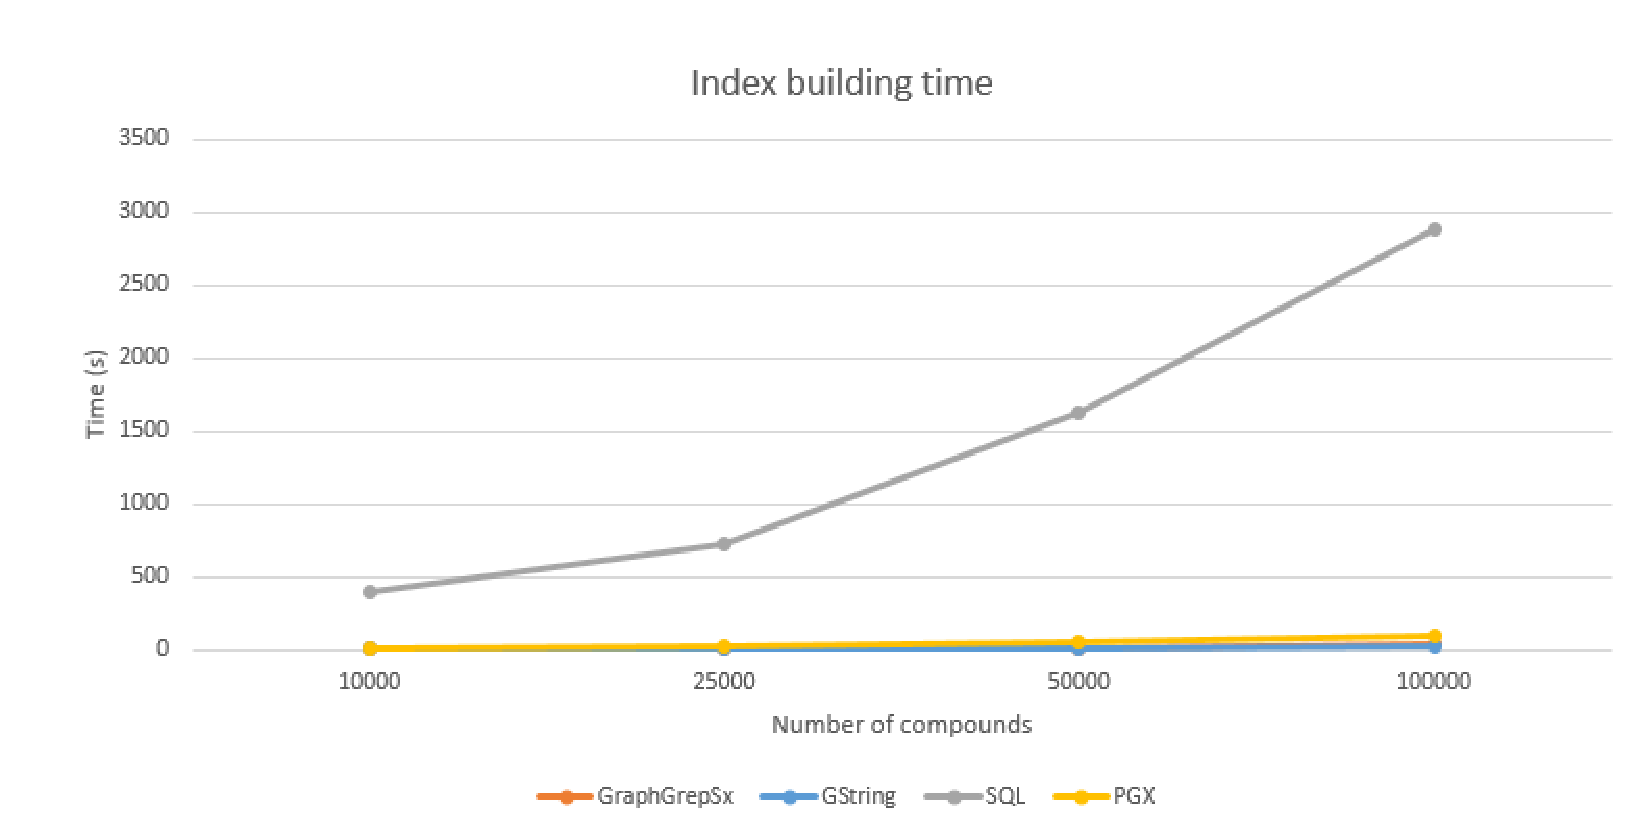
\includegraphics[width=1\textwidth]{../img/indexBuildingTime.pdf}
	\caption{Index building time}
	\label{fig:indextime}
\end{figure}

\begin{figure}[h]
	\centering
	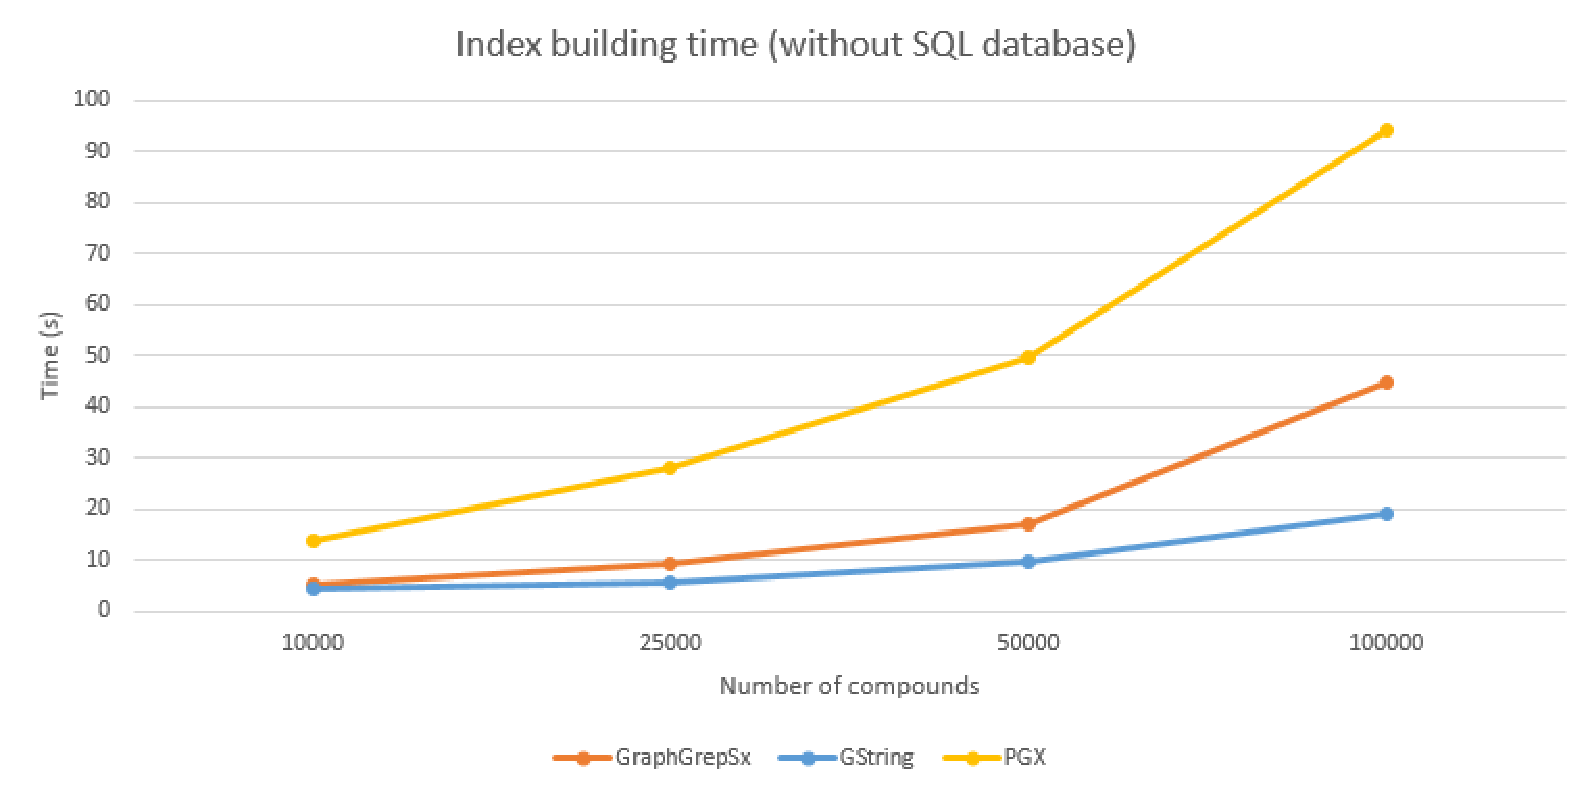
\includegraphics[width=1\textwidth]{../img/indexBuildingTimeNoSQL.pdf}
	\caption{Index building time without SQL database}
	\label{fig:indextimenosql}
\end{figure}

We may see that it is significantly slower to create the database from scratch than create just an index as it is in case of \textit{GraphGrepSX} and \textit{GString}. The results of database methods are quite convincing - SQL database creation time is 50 times slower compared to PGX. This is quite an expected result since PGX does work only in memory contrary to the SQL database which writes all the data to the disk.\\

In other two methods the difference is not so significant. \textit{GraphGrepSX} is two times slower than \textit{GString}. There might be two reasons for this observation. The first one is that for \textit{GString} we have used smaller parameter $l$ compared to \textit{GraphGrepSX}. The other explanation might be that it is worth to spend some time in condensation process, because it significantly reduces the number of distinct paths in the graph and therefore it makes the index building process faster.\\

We are not presenting the results for \textit{GIRAS}. The reason is that we were not able to get the results in a reasonable time. Even for 10 000 compounds we did not get the built index even after two days of computation. The reason is that the data set contains small structures which are substructures of many others and therefore there are not present any rare subgraphs.\\

After two days of computation for 10 000 compounds we stopped at the moment where we were missing indexing of 39 compounds and the currently searched support level was 600. In other words, these 39 compounds do not contain any subgraph (of maximal size of 8 vertices) which is rare enough to be a part of less than or equal to 600 compounds in the data set.\\

Just for verification, we tested \textit{GIRAS} on small datasets (hundreds of compounds) and the computation has finished in a reasonable time (several hours) and with expected results.\\

Because we were not able to build the \textit{GIRAS} index for our data set, we do not present the results of other metrics for this method since we had no way to measure them.

\section{Index and Data Size}
Since it is tricky to measure just the index size (and in a graph database this term does not even make sense) we have decided to measure the whole amount of memory needed for a particular method.\\

In case of \textit{GraphGrepSX} and \textit{GString} it is the memory used by the running process after the index is built and after triggered garbage collection.\\

In case of the SQL database we are querying the size of the index structure and \textbf{BONDS} table itself. The query looks as following:\\

\noindent\textbf{SELECT sum(bytes)/1024/1024 as "SIZE in MB"}\\
\phantom{x}\hspace{3ex} \textbf{FROM dba\textunderscore segments}\\
\phantom{x}\hspace{3ex} \textbf{WHERE segment\textunderscore name='BONDS/INDEX\textunderscore NAME'}\\

In case of graph database we use the \textit{getMemoryMb} method which is offered by the Java API of PGX graph representation.\\

The results are provided in Figure \ref{fig:indexsize}. What we found as an interesting observation is the size of the \textit{GString}'s index. After we saw these numbers we started to investigate what is the reason. It turned out that the premise that using the condensed graph to reduce the number od different paths is not valid. We have found out that the built index on the tested database contains more than one a half million nodes in the \textit{GString} index tree. The root node itself has almost 150 children, i.e. there are almost 150 different node types. This is a huge number compared to \textit{GraphGrepSX} which contains only 21 vertex node types.\\

\begin{figure}[h]
	\centering
	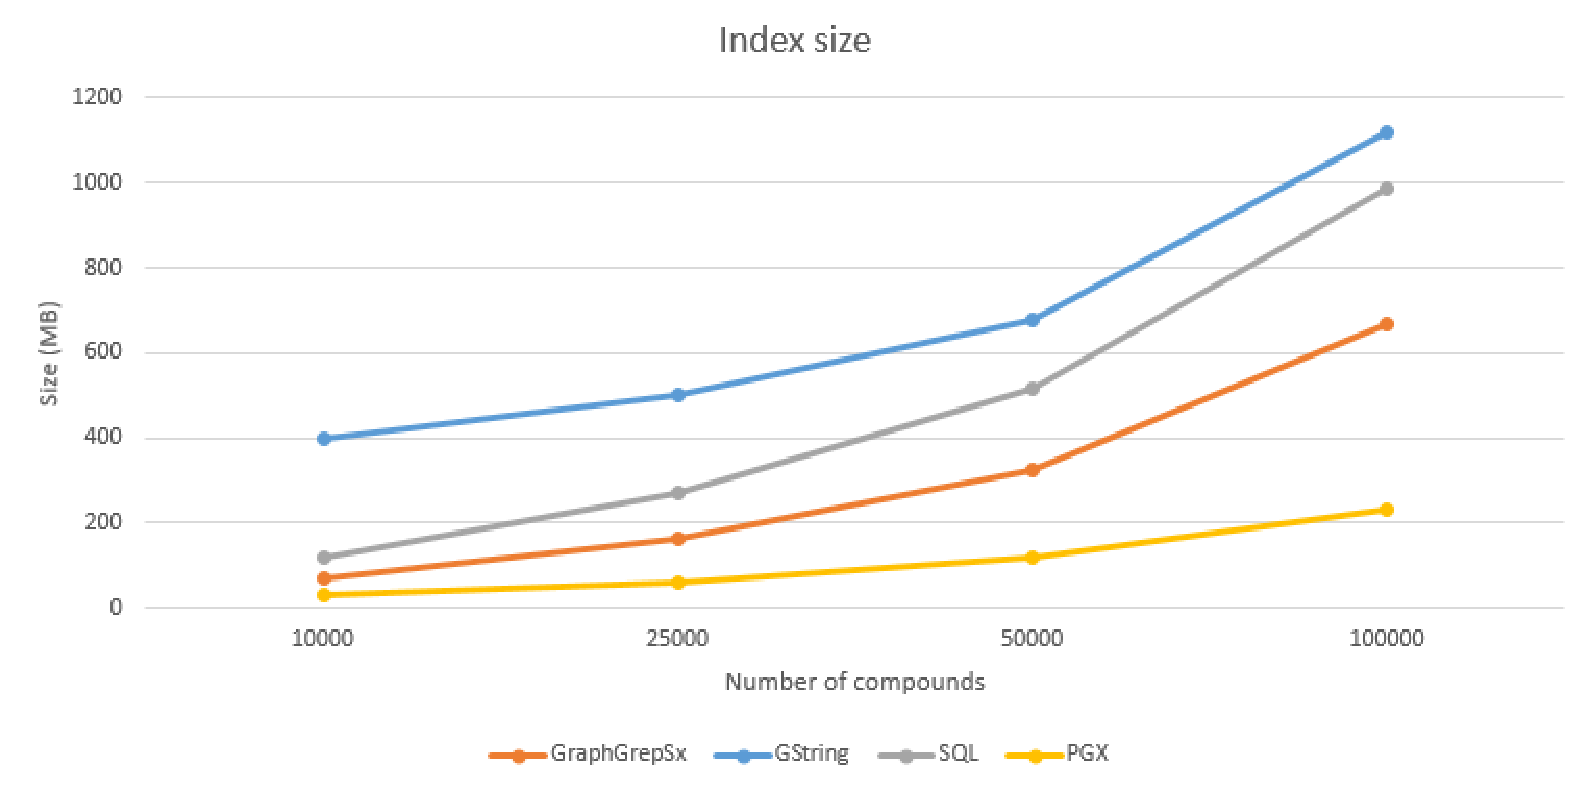
\includegraphics[width=1\textwidth]{../img/indexSize.pdf}
	\caption{Index size}
	\label{fig:indexsize}
\end{figure}

Other results are quite expected. The reason why PGX data representation is significantly smaller compared to SQL database is that PGX does not build any indices. The amount of memory consumed by SQL table representation (without the indices) is about the same as for PGX.

\section{Candidate Set Creation Time}
This metric is meaningful only for \textit{GraphGrepSX} and \textit{GString}. As we described in Chapter \ref{experimental}, the candidate set concept is not applicable to SQL and graph databases.\\

By candidate set creation we mean the time difference between the time when a query is executed and the time when we finish the index utilization for the particular query.\\

The results are provided in Figure \ref{fig:candidateset}. We can see that \textit{GString} is significantly slower compared to \textit{GraphGrepSX}. This is most probably because of the significantly bigger index size.\\

\begin{figure}[h]
	\centering
	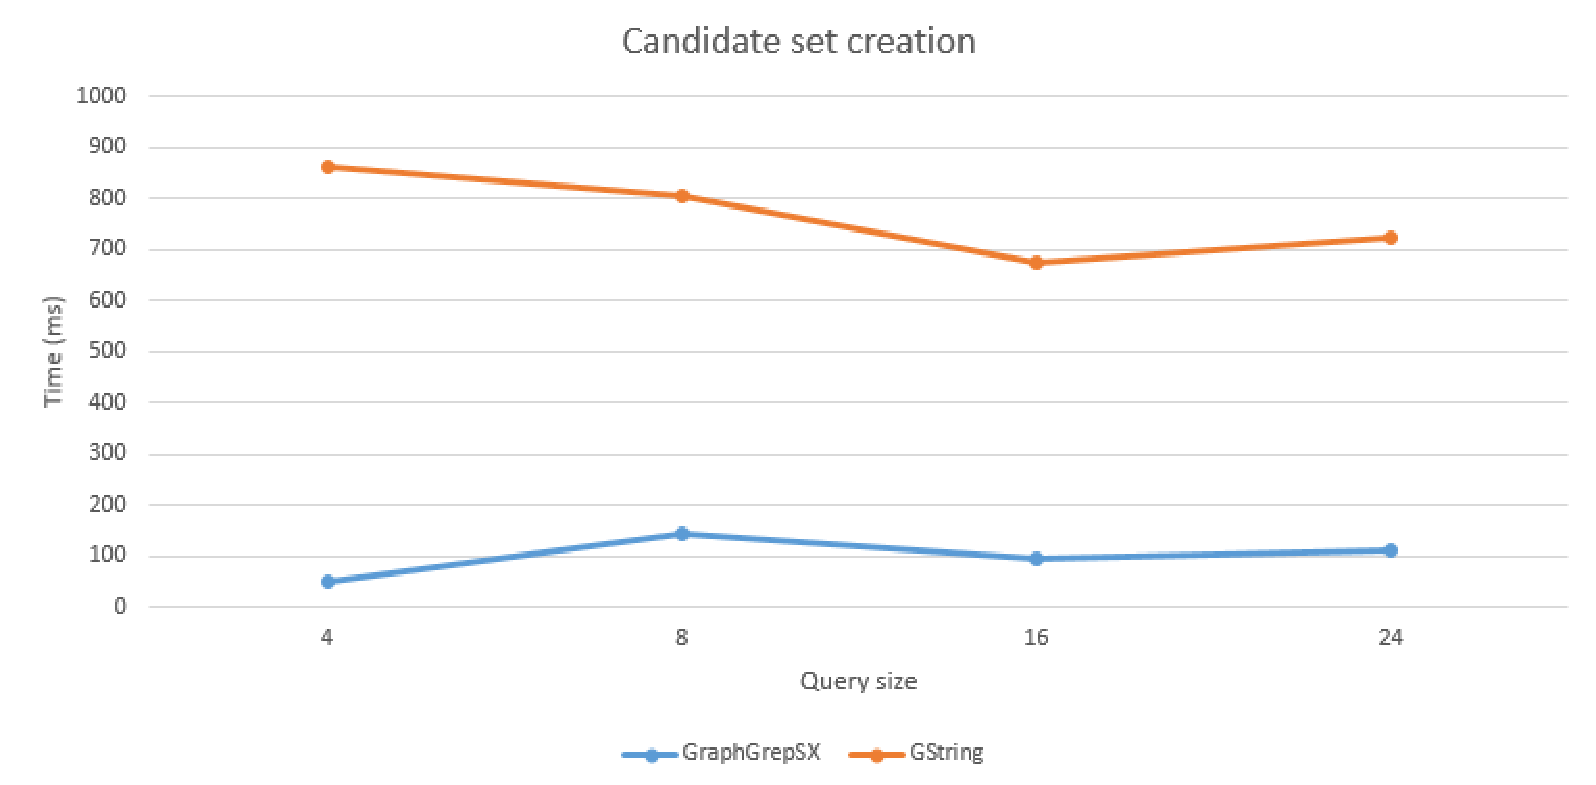
\includegraphics[width=1\textwidth]{../img/candidateSet.pdf}
	\caption{Candidate set creation time}
	\label{fig:candidateset}
\end{figure}

The other interesting fact for \textit{GString} is that due to the "stars versus paths" issue described in Section \ref{gstring} it is almost impossible to get meaningful results for large queries and therefore the candidate sets are cut down to almost empty sets.

\section{Verification Time}

Verification time does have two different meanings in this context. For methods where we create the candidate set, we understand verification time as time needed to verify the candidate set.\\

In case of SQL and graph databases, where we do not work with the candidate set concept, we understand verification time as the time needed for executing the query since we need to verify every single record in the database.\\

The results are provided in Figure \ref{fig:verification} in which we can observe several interesting outcomes.\\

\begin{figure}[h]
	\centering
	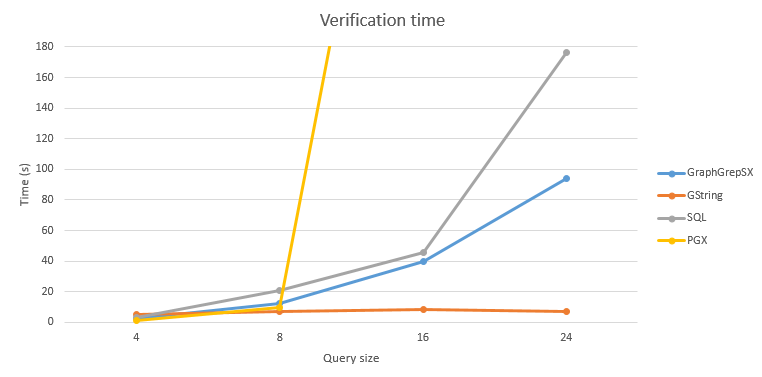
\includegraphics[width=1\textwidth]{../img/verification.png}
	\caption{Verification time}
	\label{fig:verification}
\end{figure}

At first, we can be surprised by very low numbers for verification time in case of \textit{GString}. This is caused by a significantly smaller candidate set compared to \textit{GraphGrepSX}. On the other hand, the candidate set is not smaller because of better pruning ability of \textit{GString} index, but because of the fact that \textit{GString} invalidates even the results which are valid for other methods. This was described in detail in Section \ref{gstring}.\\

The other interesting observation are the values for PGX. Although, the values for queries of sizes 4 and 8 are very good (even better than for \textit{GraphGrepSX} which is indexed) we have found out that for queries with the size bigger than 14 it is barely usable.\\

Also, we have tried to test it even on database with 1 graph with 2 vertices and 1 edge between them. We would expect that any query will be executed quickly because there is not much to compute. However, we have found that even on this small graph, big queries are very slow and the complexity grows exponentially, while query with 12 vertices took 46 seconds and query with 14 vertices took 50 minutes. Even after 3 hours of computation we were not able to get results for query with 16 vertices.\\

It seems that PGX spends a lot of time on PGQL query parsing and on creation of execution plan. We were unsure whether we did anything wrong. Luckily, the author of this thesis consulted this issue with a member of the Oracle PGX team, who confirmed that the query structure is correct and that it takes an enormous time even on Oracle internal infrastructure. We may then doubt how valid results are described in presentation \cite{pgx-neo4j} where very promising numbers even for large queries are presented.

\section{Hit Ratio of Candidate Set}
This section is only applicable for methods which create the candidate set. The metric is defined as a ratio between the candidate set size and the result set size. It measures the quality of the index, i.e. the higher the ratio is, the better results are obtained from the index.\\

The results are available in Figure \ref{fig:hitratio}. We can see that for \textit{GraphGrepSX} the efficiency of its index decreases with the query size. This is natural since the \textit{GraphGrepSX}'s index describes only paths of length up to 6. Therefore, it is expectable that with growing size of query, the accuracy will decrease, since the indexed paths cover a smaller portion of the query.\\

\begin{figure}[h]
	\centering
	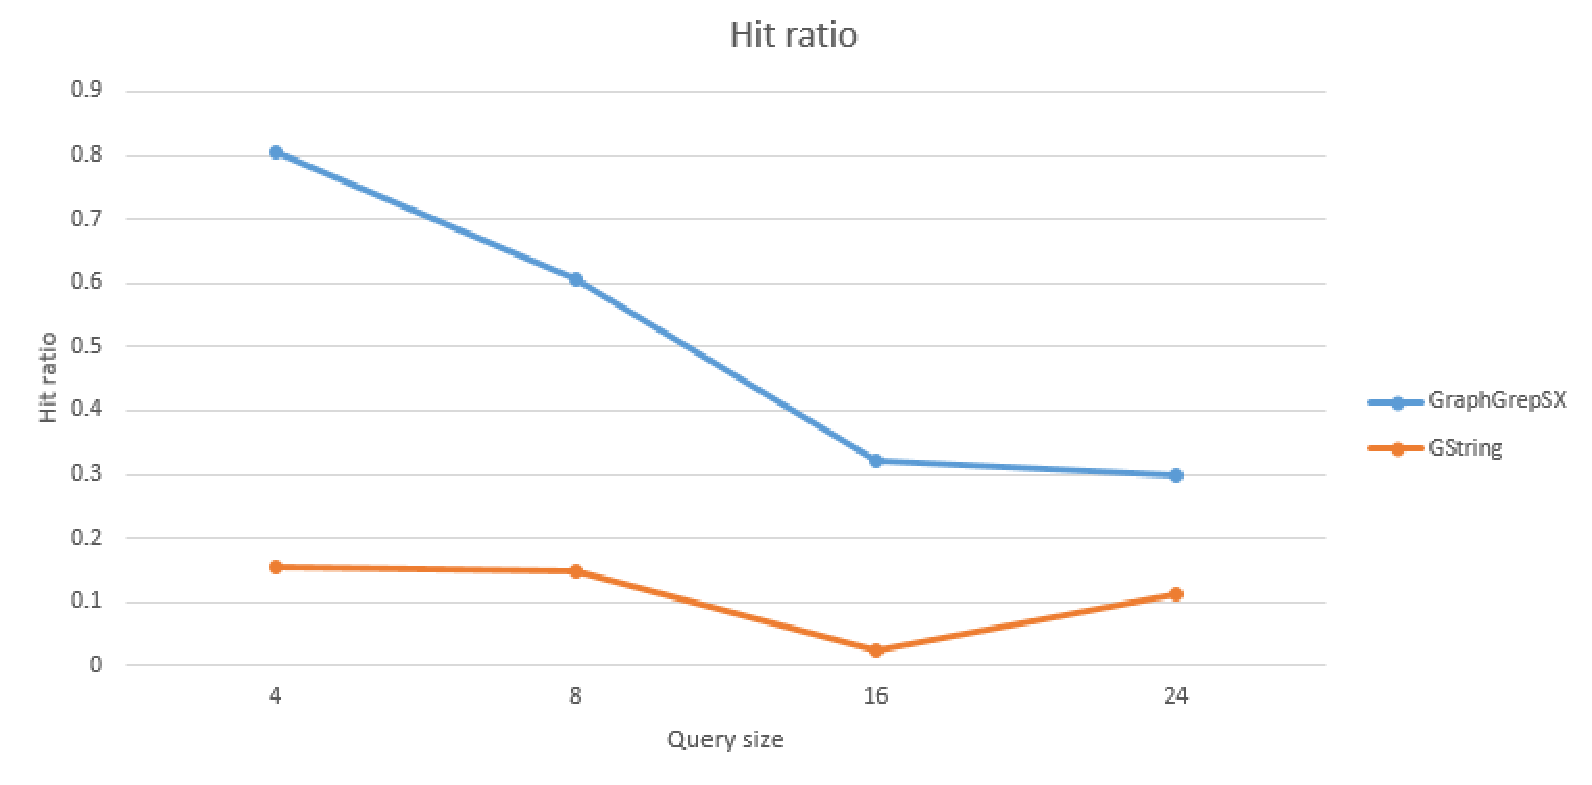
\includegraphics[width=1\textwidth]{../img/hitRatio.pdf}
	\caption{Candidate set hit ratio}
	\label{fig:hitratio}
\end{figure}

On the other hand, even queries of size 24 are not big enough to overflow the capacity of \textit{GString}. The condensed graph does not contain paths longer than 5 in these cases and therefore we would expect more or less constant hit ratio for all query sizes which matches the actual results. However, we can see that the hit ratio is significantly smaller compared to \textit{GraphGrepSX}.

\section{Query Execution Time}
In this section we describe the time results for the whole query process. It can be defined as a sum of the candidate set creation time and verification time. Note that in case of SQL and graph databases this is equal to the verification time. For the end user, this is probably the most crucial metric.\\

The results are provided in Figure \ref{fig:querytime}. The first thing we can observe is that this graph is not much different from the one in Figure \ref{fig:verification}. In other words, the time for obtaining a candidate set plays only very minor role in the total query time.\\

\begin{figure}[h]
	\centering
	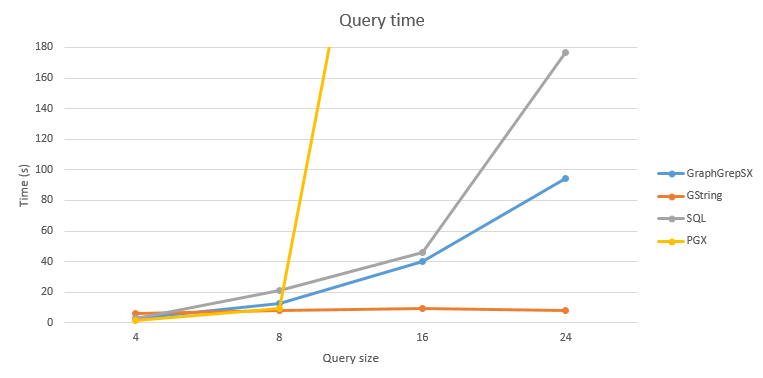
\includegraphics[width=1\textwidth]{../img/queryTime.png}
	\caption{Query time}
	\label{fig:querytime}
\end{figure}

The very good performance of \textit{GString} is a result of the fact that the result set is smaller compared to other methods. This might be confusing and a user of such method has to be aware of its limitations. On the other hand, if the user knows what are the \textit{GString} restrictions, it may be a very efficient way of querying.\\

In case of small queries, the best choice seems to be PGX. The implementation is very straight-forward and most of the work is very intuitive. Also, the implementation of PGX handler is very easily improvable to work with even much bigger data sets which cannot fit into the memory.\\

In case of the SQL database, we are quite surprised that it is a viable solution. The difference in performance times to other methods is not that significant as we would expect. Also, SQL solution is the only one which does not have to fit into memory as it is.\\

Although all other methods have their own benefits, \textit{GraphGrepSX} seems to be an overall winner. It is quite simple to implement, it has the best overall performance and reasonable index size as well as its build time.

\section{Hypotheses Results}
In this section we summarize the results of the hypotheses formulated in Section \ref{hypotheses} in Table \ref{hypothesisresults}.

\begin{table}[h]
	\centering
	\renewcommand{\arraystretch}{2.5}
	\setlength{\arrayrulewidth}{0.5mm
	}
	\begin{tabular}[h!]{|p{2cm}|p{2cm}|p{9cm}|}
		\hline
		\rowcolor{lightgray}
		Hypothesis & Result & Comments\\ \hline
		H1.1 & False & Index of \textit{GString} is significantly larger. The number of distinct nodes in case of \textit{GString} is much bigger compared to \textit{GraphGrapSX} on a real-world data set.\\ \hline
		H1.2 & Uncertain & The performance of \textit{GString} is indeed better compared to \textit{GraphGrepSX}. On the other hand, the main reason is a smaller answer set because the rules for candidate set creation are too restrictive in some cases.\\ \hline
		H2.1 & Cannot be verified & We were not able to build the \textit{GIRAS} index in a reasonable time.\\ \hline
		H2.2 & True & We were not able to build the \textit{GIRAS} index in a reasonable time even for the one tenth of the tested data set size.\\ \hline
		H3.1 & True & In general, both \textit{GraphGrepSX} and \textit{GString} perform better than SQL and PGX approaches. On the other hand, for small queries, the PGX is slightly faster. Moreover, in case of the SQL database we did expect much worse results.\\ \hline
		H3.2 & Uncertain & The hypothesis is definitely valid for small queries, in which case the performance difference is enormous. On the other hand, for larger queries PGX starts to be barely usable due to the issues with PGQL query parsing.\\ \hline
	\end{tabular}
	\caption{Hypotheses results}
	\label{hypothesisresults}
\end{table}